\section{Информационное обеспечение системы}

\subsection{Выбор средств управления данными}

Из-за сложности информационной системы была выбрана реляционная база данных для организации хранения и обработки данных.

Рассмотрим вычисление суммы лота.
Она формируемся как сумма всех смет, которые прикреплены к лоту.
Сумма сметы определяется суммой стоимостей ремонта элементов сметы.
При использовании реляционной модели доступа к данным достаточно написать два вложенных запроса, чтобы вычислить сумму лота.
При файловой модели доступа необходимо постоянно производить многочисленные операции чтения из файловой системы, что накладывает ограничения на производительность системы в целом.
Ввиду того, что система распространяется на субъект федерации, данный критерий становится критичным.

Используемая при разработке информационной системы платформа .NET поддерживает множество транспортов данных от различных СУБД до прикладной программы.

Согласно требованиям к реляционной СУБД, обозначенным в п.1.5.2 технического задания, и лицензиям заказчика, выбор предстоит сделать между Microsoft SQL Server и Oracle Database.

Обе СУБД обладают полной документацией и работают под управлением операционной системы Microsoft Windows Server 2008 R2.
Однако для простоты разработки и дальнейшей поддержки был выбран Microsoft SQL Server, так как данная система управления базами данных работает на той же платформе .NET 4 или .NET 4.5, что и разрабатываемая информационная система.

Корпорация Microsoft большое внимание уделяет нумерации серверных компонентов.
Таким образом, при использовании операционной системы версии 2008 R2 необходимо выбрать СУБД версии 2008 R2.
Этим обеспечивается полная совместимость компонентов операционной системы и системы управления базами данных.

\subsection{Проектирование базы данных}

\subsubsection{Логическая и физическая модели данных}

ER-диаграмма логической модели данных, использующая нотацию методологии IDEF1X, представлена на рисунке~\ref{img:inf-er}.

\begin{figure}[h!]
	\begin{center}
		\begin{minipage}[h]{\linewidth}
			\centering
			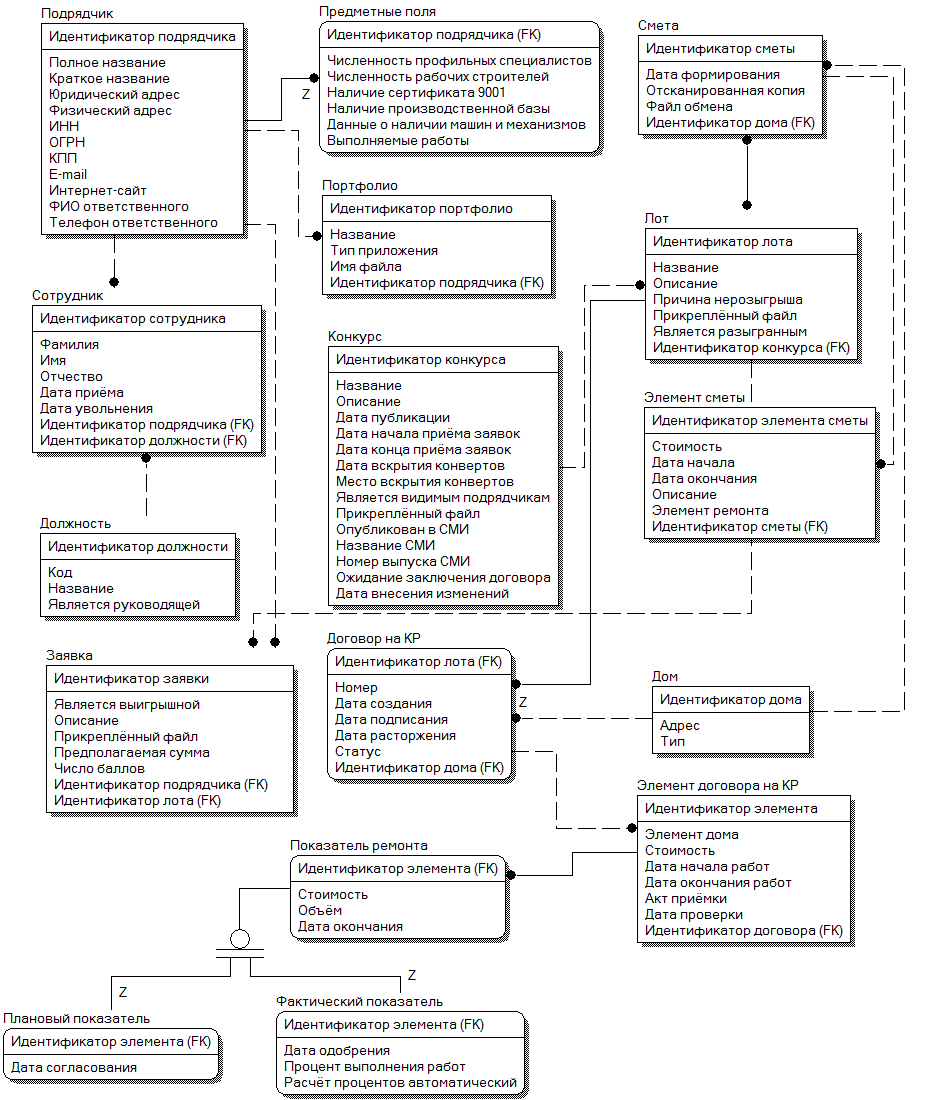
\includegraphics[width=0.85\linewidth]{images/inf-er.png}
			\caption{Логическая модель данных информационной системы}
			\label{img:inf-er}
		\end{minipage}
		\hfill
	\end{center}
\end{figure}

Описание сущностей представлено в таблице~\ref{tab:inf-entities}.

\begin{footnotesize}
\begin{longtable}[h]{|p{0.05\textwidth}|p{0.3\textwidth}|p{0.55\textwidth}|}
	\caption{\label{tab:inf-entities}Сущности логической модели данных} \\
	\hline
		\thead{№} &
		\thead{Название сущности} &
		\thead{Описание} \\
	\hline \endhead
		1 & Подрядчик & Сведения о подрядной организации \\ \hline
		2 & Предметные поля & Подробная информация о деятельности подрядчика \\ \hline
		3 & Портфолио & Элемент портфолио подрядчика \\ \hline
		4 & Сотрудник & Сведения о сотруднике подрядчика \\ \hline
		5 & Должность & Справочник должностей сотрудников \\ \hline
		6 & Дом & Сведения об объекте жилого фонда \\ \hline
		7 & Конкурс & Сведения о конкурсе на проведение КР \\ \hline
		8 & Лот & Элемент конкурса на проведение КР \\ \hline
		9 & Смета & Сведения о смете работ на дом \\ \hline
		10 & Элемент сметы & Описание необходимых работ по конструктивному элементу конкретного дома \\ \hline
		11 & Заявка & Заявка от подрядчика на розыгрыш лота \\ \hline
		12 & Договор на КР & Сведения о договоре на капитальный ремонт \\ \hline
		13 & Элемент договора на КР & Часть договора, описывающая конкретную часть ремонта \\ \hline
		14 & Плановый показатель & Сведения о планируемом ходе ремонта элемента дома \\ \hline
		15 & Фактический показатель & Сведения о фактическом ходе ремонта элемента дома \\ \hline
		16 & Показатель ремонта & Сведения о показателях элементов ремонта дома \\ \hline
\end{longtable}
\end{footnotesize}

Список сотрудников включён в логическую модель данных, так как содержание информации о сотрудниках каждой подрядной организации является требованием заказчика.
Также это требование отражено в техническом задании.

Ниже представлены таблицы с атрибутами сущностей.
Дополнительно в таблицах приведено сопоставление логической и физической модели данных.
Названия таблиц и полей, сопоставленных с соответствующими сущностями и атрибутами, указаны в фигурных скобках.

Атрибуты сущности [Подрядчик] представлены в таблице~\ref{tab:inf-contractor}.

\begin{footnotesize}
\begin{longtable}[h]{|p{0.05\textwidth}|p{0.3\textwidth}|p{0.2\textwidth}|p{0.35\textwidth}|}
	\caption{\label{tab:inf-contractor}Атрибуты сущности [Подрядчик] и поля таблицы \{Contractor\}} \\
	\hline
		\thead{№} &
		\thead{Название атрибута/поля} &
		\thead{Тип} &
		\thead{Описание} \\
	\hline
		\theadnum{1} & \theadnum{2} & \theadnum{3} & \theadnum{4} \\
	\hline \endfirsthead
	\hline
		\theadnum{1} & \theadnum{2} & \theadnum{3} & \theadnum{4} \\
	\hline \endhead
	1 & Идентификатор подрядчика \par \{Id\} & Числовой \par \{int\} & Идентификатор подрядной организации \\ \hline
	2 & Полное название \par \{FullName\} & Текстовый \par \{nvarchar(500)\} & Полное название подрядчика \\ \hline
	3 & Краткое название \par \{ShortName\} & Текстовый \par \{nvarchar(200)\} & Краткое название подрядчика \\ \hline
	4 & Юридический адрес \par \{LegalAddress\} & Текстовый \par \{nvarchar(500)\} & Юридический адрес подрядчика \\ \hline
	5 & Физический адрес \par \{PhysicalAddress\} & Текстовый \par \{nvarchar(500)\} & Физический адрес подрядчика \\ \hline
	6 & ИНН \par \{INN\} & Текстовый \par \{nvarchar(20)\} & ИНН подрядчика \\ \hline
	7 & ОГРН \par \{OGRN\} & Текстовый \par \{nvarchar(15)\} & ОГРН подрядчика \\ \hline
	8 & КПП \par \{KPP\} & Текстовый \par \{nvarchar(20)\} & КПП подрядчика \\ \hline
	9 & E-mail \par \{Email\} & Текстовый \par \{nvarchar(150)\} & E-mail подрядчика для связи \\ \hline
	10 & Интернет-сайт \par \{Site\} & Текстовый \par \{nvarchar(150)\} & Адрес веб-сайта подрядчика \\ \hline
	11 & ФИО ответственного \par \{ResponsibleName\} & Текстовый \par \{nvarchar(200)\} & ФИО ответственного лица за участие в конкурсах \\ \hline
	12 & Телефон ответственного \par \{ResponsiblePhone\} & Текстовый \par \{nvarchar(50)\} & Телефон ответственного лица за участие в конкурсах \\ \hline
\end{longtable}
\end{footnotesize}

В данной сущности умышленно нарушается НФБК для увеличения доступа к данным.
При процессе нормализации ФИО и Телефон ответственного можно вынести в отдельную сущность, но это усложнит схему данных информационной системы, увеличив число запросов к БД.
К тому же, в данном случае в информационной системе нигде не идёт работа с ответственным отдельно от подрядчика.

Атрибуты сущности [Предметные поля] представлены в таблице~\ref{tab:inf-contractorinfo}.

\begin{footnotesize}
\begin{longtable}[h]{|p{0.05\textwidth}|p{0.3\textwidth}|p{0.2\textwidth}|p{0.35\textwidth}|}
	\caption{\label{tab:inf-contractorinfo}Атрибуты сущности [Предметные поля] и поля таблицы \{ContractorInformation\}} \\
	\hline
		\thead{№} &
		\thead{Название атрибута/поля} &
		\thead{Тип} &
		\thead{Описание} \\
	\hline
		\theadnum{1} & \theadnum{2} & \theadnum{3} & \theadnum{4} \\
	\hline \endfirsthead
	\hline
		\theadnum{1} & \theadnum{2} & \theadnum{3} & \theadnum{4} \\
	\hline \endhead
	1 & Идентификатор подрядчика \par \{Id\} & Числовой \par \{int\} & Связь с подрядчиком \\ \hline
	2 & Численность профильных специалистов \par \{ProfileExpertsNumber\} & Числовой \par \{int\} & Численность специалистов по капитальному ремонту \\ \hline
	3 & Численность рабочих строителей \par \{BuildersNumber\} & Числовой \par \{int\} & Численность строителей, которые могут выполнять КР \\ \hline
	4 & Наличие сертификата 9001 \par \{HasIso9001Certificate\} & Логический \par \{bool\} & Наличие у подрядчика сертификата ISO 9001:2000 \\ \hline
	5 & Наличие производственной базы \par \{HasProductionBase\} & Логический \par \{bool\} & Возможность производства материалов у подрядчика \\ \hline
	6 & Данные о наличии машин и механизмов \par \{MachineryDescription\} & Текстовый \par \{nvarchar(max)\} & Данные о наличии строительной техники у подрядчика \\ \hline
	7 & Выполняемые работы \par \{WorkDescription\} & Текстовый \par \{nvarchar(max)\} & Сведения о работах текущих подрядчика \\ \hline
\end{longtable}
\end{footnotesize}

Атрибуты сущности [Портфолио] представлены в таблице~\ref{tab:inf-portfolio}.

\begin{footnotesize}
\begin{longtable}[h]{|p{0.05\textwidth}|p{0.3\textwidth}|p{0.2\textwidth}|p{0.35\textwidth}|}
	\caption{\label{tab:inf-portfolio}Атрибуты сущности [Портфолио] и поля таблицы \{Portfolio\}} \\
	\hline
		\thead{№} &
		\thead{Название атрибута/поля} &
		\thead{Тип} &
		\thead{Описание} \\
	\hline
		\theadnum{1} & \theadnum{2} & \theadnum{3} & \theadnum{4} \\
	\hline \endfirsthead
	\hline
		\theadnum{1} & \theadnum{2} & \theadnum{3} & \theadnum{4} \\
	\hline \endhead
	1 & Идентификатор портфолио \par \{Id\} & Числовой \par \{int\} & Идентификатор записи портфолио подрядчика \\ \hline
	2 & Название \par \{Name\} & Текстовый \par \{nvarchar(200)\} & Название записи портфолио \\ \hline
	3 & Тип приложения \par \{DocumentType\} & Справочник \par \{int\} & Тип записи портфолио (изображение, документ) \\ \hline
	4 & Имя файла \par \{FileName\} & Текстовый \par \{nvarchar(100)\} & Имя файла с приложением в ФС \\ \hline
	5 & Идентификатор подрядчика \par \{OrganizationId\} & Числовой \par \{int\} & Связь с подрядчиком \\ \hline
\end{longtable}
\end{footnotesize}

Атрибуты сущности [Сотрудник] представлены в таблице~\ref{tab:inf-employee}.

\begin{footnotesize}
\begin{longtable}[h]{|p{0.05\textwidth}|p{0.3\textwidth}|p{0.2\textwidth}|p{0.35\textwidth}|}
	\caption{\label{tab:inf-employee}Атрибуты сущности [Сотрудник] и поля таблицы \{Employee\}} \\
	\hline
		\thead{№} &
		\thead{Название атрибута/поля} &
		\thead{Тип} &
		\thead{Описание} \\
	\hline
		\theadnum{1} & \theadnum{2} & \theadnum{3} & \theadnum{4} \\
	\hline \endfirsthead
	\hline
		\theadnum{1} & \theadnum{2} & \theadnum{3} & \theadnum{4} \\
	\hline \endhead
	1 & Идентификатор сотрудника \par \{Id\} & Числовой \par \{int\} & Идентификатор записи о сотруднике подрядчика \\ \hline
	2 & Фамилия \par \{LastName\} & Текстовый \par \{nvarchar(100)\} & Фамилия сотрудника \\ \hline
	3 & Имя \par \{FirstName\} & Текстовый \par \{nvarchar(100)\} & Имя сотрудника \\ \hline
	4 & Отчество \par \{MiddleName\} & Текстовый \par \{nvarchar(100)\} & Отчество сотрудника \\ \hline
	5 & Дата приёма \par \{DateStart\} & Дата \par \{datetime\} & Дата приёма сотрудника на должность \\ \hline
	6 & Дата увольнения \par \{DateEnd\} & Дата \par \{datetime\} & Дата освобождения от должности \\ \hline
	7 & Идентификатор подрядчика \par \{OrganizationId\} & Числовой \par \{int\} & Связь с подрядчиком \\ \hline
	8 & Идентификатор должности \par \{PositionId\} & Числовой \par \{int\} & Связь с должностью сотрудника	\\ \hline
\end{longtable}
\end{footnotesize}

Атрибуты сущности [Должность] представлены в таблице~\ref{tab:inf-employeePosition}.

\begin{footnotesize}
\begin{longtable}[h]{|p{0.05\textwidth}|p{0.3\textwidth}|p{0.2\textwidth}|p{0.35\textwidth}|}
	\caption{\label{tab:inf-employeePosition}Атрибуты сущности [Должность] и поля таблицы \{EmployeePosition\}} \\
	\hline
		\thead{№} &
		\thead{Название атрибута/поля} &
		\thead{Тип} &
		\thead{Описание} \\
	\hline
		\theadnum{1} & \theadnum{2} & \theadnum{3} & \theadnum{4} \\
	\hline \endfirsthead
	\hline
		\theadnum{1} & \theadnum{2} & \theadnum{3} & \theadnum{4} \\
	\hline \endhead
	1 & Идентификатор должности \par \{Id\} & Числовой \par \{int\} & Идентификатор должностей сотрудников \\ \hline
	2 & Код \par \{Code\} & Текстовый \par \{nvarchar(50)\} & Кодовое название должности \\ \hline
	3 & Название \par \{Name\} & Текстовый \par \{nvarchar(200)\} & Название должности \\ \hline
	4 & Является руководящей \par \{CanBeDirector\} & Логический \par \{bit\} & Является ли должность руководящей \\ \hline
\end{longtable}
\end{footnotesize}

Атрибуты сущности [Дом] представлены в таблице~\ref{tab:inf-object}.

\begin{footnotesize}
\begin{longtable}[h]{|p{0.05\textwidth}|p{0.3\textwidth}|p{0.2\textwidth}|p{0.35\textwidth}|}
	\caption{\label{tab:inf-object}Атрибуты сущности [Дом] и поля таблицы \{cmn\$Object\}} \\
	\hline
		\thead{№} &
		\thead{Название атрибута/поля} &
		\thead{Тип} &
		\thead{Описание} \\
	\hline
		\theadnum{1} & \theadnum{2} & \theadnum{3} & \theadnum{4} \\
	\hline \endfirsthead
	\hline
		\theadnum{1} & \theadnum{2} & \theadnum{3} & \theadnum{4} \\
	\hline \endhead
	1 & Идентификатор дома \par \{Id\} & Числовой \par \{Id\} & Идентификатор дома \\ \hline
	2 & Адрес \par \{StructureAddrText\} & Текстовый \par \{nvarchar(500)\} & Адрес дома \\ \hline
	3 & Тип \par \{ObjectType\} & Справочник \par \{int\} & Тип дома \\ \hline
\end{longtable}
\end{footnotesize}

В таблице выше показаны только те поля, которые необходимы для информационной системы.
Фактически в данной таблице содержится более 15 полей.

Атрибуты сущности [Конкурс] представлены в таблице~\ref{tab:inf-contest}.

\begin{footnotesize}
\begin{longtable}[h]{|p{0.05\textwidth}|p{0.3\textwidth}|p{0.2\textwidth}|p{0.35\textwidth}|}
	\caption{\label{tab:inf-contest}Атрибуты сущности [Конкурс] и поля таблицы \{Contest\}} \\
	\hline
		\thead{№} &
		\thead{Название атрибута/поля} &
		\thead{Тип} &
		\thead{Описание} \\
	\hline
		\theadnum{1} & \theadnum{2} & \theadnum{3} & \theadnum{4} \\
	\hline \endfirsthead
	\hline
		\theadnum{1} & \theadnum{2} & \theadnum{3} & \theadnum{4} \\
	\hline \endhead
	1 & Идентификатор конкурса \par \{Id\} & Числовой \par \{int\} & Идентификатор конкурса на КР \\ \hline
	2 & Название \par \{Name\} & Текстовый \par \{nvarchar(100)\} & Название конкурса \\ \hline
	3 & Описание \par \{Description\} & Текстовый \par \{nvarchar(max)\} & Краткое описание конкурса \\ \hline
	4 & Дата публикации \par \{DatePublish\} & Дата \par \{datetime2\} & Дата выхода СМИ с информацией о конкурсе \\ \hline
	5 & Дата начала приёма заявок \par \{DateStart\} & Дата \par \{datetime2\} & Дата начала приёма заявок на розыгрыш лотов конкурса \\ \hline
	6 & Дата конца приёма заявок \par \{DateEnd\} & Дата \par \{datetime2\} & Дата конца приёма заявок на розыгрыш лотов конкурса \\ \hline
	7 & Дата вскрытия конвертов \par \{DateOpening\} & ДатаВремя \par \{datetime2(2)\} & Дата и время вскрытия конвертов с заявками подрядчиков \\ \hline
	8 & Место вскрытия конвертов \par \{PlaceOpening\} & Текстовый \par \{nvarchar(200)\} & Место вскрытия конвертов с заявками подрядчиков \\ \hline
	9 & Является видимым подрядчикам \par \{IsVisible\} & Логический \par \{bit\} & Является ли конкурс видимым на портале подрядчиков \\ \hline
	10 & Прикреплённый файл \par \{FileName\} & Текстовый \par \{nvarchar(100)\} & Путь до прикреплённого к конкурсу файлу в ФС \\ \hline
	11 & Опубликован в СМИ \par \{IsPublished\} & Логический \par \{bit\} & Размещена ли информация о конкурсе в СМИ \\ \hline
	12 & Название СМИ \par \{NamePublish\} & Текстовый \par \{nvarchar(100)\} & Название СМИ, в котором опубликована информация о конкурсе \\ \hline
	13 & Номер выпуска СМИ \par \{NumberPublish\} & Текстовый \par \{nvarchar(10)\} & Номер выпуска СМИ, в котором опубликована информация о конкурсе \\ \hline
	14 & Ожидание заключение договора \par \{ContractDaysLimit\} & Денежный \par \{money\} & Срок (указан в днях), в течение которого на разыгранный в рамках конкурса лот должен быть заключен контракт \\ \hline
	15 & Дата внесения изменений \par \{Updated\} & ДатаВремя \par \{datetime2(2)\} & Дата и время внесения последних изменений в сведения о конкурсе \\ \hline
\end{longtable}
\end{footnotesize}

Атрибуты сущности [Лот] представлены в таблице~\ref{tab:inf-lot}.

\begin{footnotesize}
\begin{longtable}[h]{|p{0.05\textwidth}|p{0.3\textwidth}|p{0.2\textwidth}|p{0.35\textwidth}|}
	\caption{\label{tab:inf-lot}Атрибуты сущности [Лот] и поля таблицы \{Lot\}} \\
	\hline
		\thead{№} &
		\thead{Название атрибута/поля} &
		\thead{Тип} &
		\thead{Описание} \\
	\hline
		\theadnum{1} & \theadnum{2} & \theadnum{3} & \theadnum{4} \\
	\hline \endfirsthead
	\hline
		\theadnum{1} & \theadnum{2} & \theadnum{3} & \theadnum{4} \\
	\hline \endhead
	1 & Идентификатор лота \par \{Id\} & Числовой \par \{int\} & Идентификатор лота конкурса \\ \hline
	2 & Название \par \{Name\} & Текстовый \par \{nvarchar(100)\} & Название лота \\ \hline
	3 & Описание \par \{Description\} & Текстовый \par \{nvarchar(max)\} & Краткое описание лота \\ \hline
	4 & Причина нерозгрыша \par \{Reason\} & Текстовый \par \{nvarchar(255)\} & Причина, по которой лот был не разыгран \\ \hline
	5 & Прикреплённый файл \par \{FileName\} & Текстовый \par \{nvarchar(100)\} & Имя прикреплённого файла в ФС \\ \hline
	6 & Является разыгранным \par \{Status\} & Логический \par \{bit\} & Статус розыгрыша конкурса \\ \hline
	7 & Идентификатор конкурса \par \{ContestId\} & Числовой \par \{int\} & Связь с конкурсом на КР \\ \hline
\end{longtable}
\end{footnotesize}

Атрибуты сущности [Смета] представлены в таблице~\ref{tab:inf-costEstimation}.

\begin{footnotesize}
\begin{longtable}[h]{|p{0.05\textwidth}|p{0.3\textwidth}|p{0.2\textwidth}|p{0.35\textwidth}|}
	\caption{\label{tab:inf-costEstimation}Атрибуты сущности [Смета] и поля таблицы \{CostEstimation\}} \\
	\hline
		\thead{№} &
		\thead{Название атрибута/поля} &
		\thead{Тип} &
		\thead{Описание} \\
	\hline
		\theadnum{1} & \theadnum{2} & \theadnum{3} & \theadnum{4} \\
	\hline \endfirsthead
	\hline
		\theadnum{1} & \theadnum{2} & \theadnum{3} & \theadnum{4} \\
	\hline \endhead
	1 & Идентификатор сметы \par \{Id\} & Числовой \par \{int\} & Идентификатор сметы на работы по КР \\ \hline
	2 & Дата формирования \par \{Date\}] & Дата \par \{datetime2\} & Дата формирования сметы \\ \hline
	3 & Отсканированная копия \par \{ScanFileName\} & Текстовый \par \{nvarchar(100)\} & Путь до файла с отсканированной копией в ФС \\ \hline
	4 & Файл обмена \par \{ChangeFileName\} & Текстовый \par \{nvarchar(100)\} & Путь до файла обмена типа АПРС 1.10 \\ \hline
	5 & Идентификатор дома \par \{ObjectId\} & Числовой \par \{int\} & Связь с домом \\ \hline
\end{longtable}
\end{footnotesize}

Атрибуты сущности [Элемент сметы] представлены в таблице~\ref{tab:inf-costEstimationElement}.

\begin{footnotesize}
\begin{longtable}[h]{|p{0.05\textwidth}|p{0.3\textwidth}|p{0.2\textwidth}|p{0.35\textwidth}|}
	\caption{\label{tab:inf-costEstimationElement}Атрибуты сущности [Элемент сметы] и поля таблицы \{CostEstimationElement\}} \\
	\hline
		\thead{№} &
		\thead{Название атрибута/поля} &
		\thead{Тип} &
		\thead{Описание} \\
	\hline
		\theadnum{1} & \theadnum{2} & \theadnum{3} & \theadnum{4} \\
	\hline \endfirsthead
	\hline
		\theadnum{1} & \theadnum{2} & \theadnum{3} & \theadnum{4} \\
	\hline \endhead
	1 & Идентификатор элемента сметы \par \{Id\} & Числовой \par \{int\} & Идентификатор элемента сметы \\ \hline
	2 & Стоимость \par \{Sum\} & Денежный \par \{money\} & Стоимость ремонта элемента сметы \\ \hline
	3 & Дата начала \par \{DateStart\} & Дата \par \{datetime2\} & Предположительная дата начала ремонта \\ \hline
	4 & Дата окончания \par \{DateEnd\} & Дата \par \{datetime2\} & Предположительная дата окончания ремонта \\ \hline
	5 & Описание \par \{Description\} & Текстовый \par \{nvarchar(max)\} & Краткое описание элемента сметы \\ \hline
	6 & Элемент ремонта \par \{ElementName\} & Текстовый \par \{nvarchar(100)\} & Название вида работ по ремонту дома \\ \hline
	7 & Идентификатор сметы \par \{CostEstimationId\} & Числовой \par \{int\} & Связь со сметой \\ \hline
\end{longtable}
\end{footnotesize}

Атрибуты сущности [Заявка] представлены в таблице~\ref{tab:inf-bid}.

\begin{footnotesize}
\begin{longtable}[h]{|p{0.05\textwidth}|p{0.3\textwidth}|p{0.2\textwidth}|p{0.35\textwidth}|}
	\caption{\label{tab:inf-bid}Атрибуты сущности [Заявка] и поля таблицы \{Bid\}} \\
	\hline
		\thead{№} &
		\thead{Название атрибута/поля} &
		\thead{Тип} &
		\thead{Описание} \\
	\hline
		\theadnum{1} & \theadnum{2} & \theadnum{3} & \theadnum{4} \\
	\hline \endfirsthead
	\hline
		\theadnum{1} & \theadnum{2} & \theadnum{3} & \theadnum{4} \\
	\hline \endhead
	1 & Идентификатор заявки \par \{Id\} & Числовой \par \{int\} & Идентификатор заявки от подрядчика на розыгрыш лота конкурса \\ \hline
	2 & Является выигрышной \par \{IsWon\} & Логический \par \{bit\} & Выиграла ли заявка в розыгрыше \\ \hline
	3 & Описание \par \{Comment\} & Текстовый \par \{nvarchar(max)\} & Краткое описание заявки \\ \hline
	4 & Прикреплённый файл \par \{FileName\} & Текстовый \par \{nvarchar(100)\} & Путь до прикреплённого к заявке файла \\ \hline
	5 & Предполагаемая сумма \par \{Sum\} & Денежный \par \{money\} & Сумма ремонта согласно заявке \\ \hline
	6 & Число баллов \par \{Points\} & Числовой \par \{int\} & Число баллов заявки \\ \hline
	7 & Идентификатор подрядчика \par \{Organizationid\} & Числовой \par \{int\} & Связь с подрядчиком \\ \hline
	8 & Идентификатор лота \par \{LotId\} & Числовой \par \{int\} & Связь с лотом \\ \hline
\end{longtable}
\end{footnotesize}

Атрибуты сущности [Договор на КР] представлены в таблице~\ref{tab:inf-contractOnWork}.

\begin{footnotesize}
\begin{longtable}[h]{|p{0.05\textwidth}|p{0.3\textwidth}|p{0.2\textwidth}|p{0.35\textwidth}|}
	\caption{\label{tab:inf-contractOnWork}Атрибуты сущности [Договор на КР] и поля таблицы \{ContractOnWork\}} \\
	\hline
		\thead{№} &
		\thead{Название атрибута/поля} &
		\thead{Тип} &
		\thead{Описание} \\
	\hline
		\theadnum{1} & \theadnum{2} & \theadnum{3} & \theadnum{4} \\
	\hline \endfirsthead
	\hline
		\theadnum{1} & \theadnum{2} & \theadnum{3} & \theadnum{4} \\
	\hline \endhead
	1 & Идентификатор лота \par \{Id\} & Числовой \par \{int\} & Связь с лотом \\ \hline
	2 & Номер \par \{Number\} & Текстовый \par \{nvarchar(100)\} & Номер договора на КР \\ \hline
	3 & Дата создания \par \{DateCreating\} & ДатаВремя \par \{datetime2(2)\} & Дата создания договора в ИС \\ \hline
	4 & Дата подписания \par \{DateSignature\} & Дата \par \{date\} & Дата подписания договора сторонами \\ \hline
	5 & Дата расторжения \par \{DateTermination\} & Дата \par \{date\} & Дата расторжения договора на КР \\ \hline
	6 & Статус \par \{StatusId\} & Справочник \par \{int\} & Статус договора на КР \\ \hline
	7 & Идентификатор дома \par \{ObjectId\} & Числовой \par \{int\} & Связь с домом \\ \hline
\end{longtable}
\end{footnotesize}

Атрибуты сущности [Элемент договора на КР] представлены в таблице~\ref{tab:inf-contractOnWorkElement}.

\begin{footnotesize}
\begin{longtable}[h]{|p{0.05\textwidth}|p{0.3\textwidth}|p{0.2\textwidth}|p{0.35\textwidth}|}
	\caption{\label{tab:inf-contractOnWorkElement}Атрибуты сущности [Элемент договора на КР] и поля таблицы \{ContractOnWorkElement\}} \\
	\hline
		\thead{№} &
		\thead{Название атрибута/поля} &
		\thead{Тип} &
		\thead{Описание} \\
	\hline
		\theadnum{1} & \theadnum{2} & \theadnum{3} & \theadnum{4} \\
	\hline \endfirsthead
	\hline
		\theadnum{1} & \theadnum{2} & \theadnum{3} & \theadnum{4} \\
	\hline \endhead
	1 & Идентификатор элемента \par \{Id\} & Числовой \par \{int\} & Идентификатор элемента договора \\ \hline
	2 & Элемент дома \par \{ElementName\} & Текстовый \par \{nvarchar(100)\} & Конструктивный элемент дома \\ \hline
	3 & Стоимость \par \{Sum\} & Денежный \par \{money\} & Стоимость ремонта элемента договора \\ \hline
	4 & Дата начала работ \par \{DateStart\} & Дата \par \{datetime2\} & Дата начала работ по договору на КР \\ \hline
	5 & Дата окончания работ \par \{DateEnd\} & Дата \par \{datetime2\} & Дата окончания работ по договору на КР \\ \hline
	6 & Акт приёмки \par \{AcceptanceReport\} & Текстовый \par \{nvarchar(100)\} & Путь до файла с отсканированном файлом приёмки работ по элементу договора \\ \hline
	7 & Дата проверки \par \{DateChecking\} & Дата \par \{datetime2\} & Дата проверки элемента договора \\ \hline
\end{longtable}
\end{footnotesize}

Атрибуты сущности [Плановый показатель] представлены в таблице~\ref{tab:inf-contractOnWorkPlan}.

\begin{footnotesize}
\begin{longtable}[h]{|p{0.05\textwidth}|p{0.3\textwidth}|p{0.2\textwidth}|p{0.35\textwidth}|}
	\caption{\label{tab:inf-contractOnWorkPlan}Атрибуты сущности [Плановый показатель] и поля таблицы \{ContractOnWorkPlan\}} \\
	\hline
		\thead{№} &
		\thead{Название атрибута/поля} &
		\thead{Тип} &
		\thead{Описание} \\
	\hline
		\theadnum{1} & \theadnum{2} & \theadnum{3} & \theadnum{4} \\
	\hline \endfirsthead
	\hline
		\theadnum{1} & \theadnum{2} & \theadnum{3} & \theadnum{4} \\
	\hline \endhead
	1 & Идентификатор элемента \par \{Id\} & Числовой \par \{int\} & Идентификатор элемента договора на КР \\ \hline
	2 & Дата согласования \par \{DateChecking\} & Дата \par \{datetime2\} & Дата согласования плана ремонта \\ \hline
\end{longtable}
\end{footnotesize}

Атрибуты сущности [Фактический показатель] представлены в таблице~\ref{tab:inf-contractOnWorkFact}.

\begin{footnotesize}
\begin{longtable}[h]{|p{0.05\textwidth}|p{0.3\textwidth}|p{0.2\textwidth}|p{0.35\textwidth}|}
	\caption{\label{tab:inf-contractOnWorkFact}Атрибуты сущности [Фактический показатель] и поля таблицы \{ContractOnWorkFact\}} \\
	\hline
		\thead{№} &
		\thead{Название атрибута/поля} &
		\thead{Тип} &
		\thead{Описание} \\
	\hline
		\theadnum{1} & \theadnum{2} & \theadnum{3} & \theadnum{4} \\
	\hline \endfirsthead
	\hline
		\theadnum{1} & \theadnum{2} & \theadnum{3} & \theadnum{4} \\
	\hline \endhead
	1 & Идентификатор элемента \par \{Id\} & Числовой \par \{int\} & Идентификатор элемента договора на КР \\ \hline
	2 & Дата одобрения \par \{DateApproved\} & Дата \par \{datetime2\} & Дата одобрения фактических значений ремонта по элементу договора на КР \\ \hline
	3 & Процент выполнения работ \par \{Completed\} & Числовой \par \{decimal(5,2)\} & Текущий прогресс выполнения ремонта \\ \hline
	4 & Расчёт процентов автоматический \par \{IsAutoCompleted\} & Логический \par \{bit\} & Является ли расчёт процентов автоматическим \\ \hline
\end{longtable}
\end{footnotesize}

Атрибуты сущности [Показатель ремонта] представлены в таблице~\ref{tab:inf-contractOnWorkPF}.

\begin{footnotesize}
\begin{longtable}[h]{|p{0.05\textwidth}|p{0.3\textwidth}|p{0.2\textwidth}|p{0.35\textwidth}|}
	\caption{\label{tab:inf-contractOnWorkPF}Атрибуты сущности [Показатель ремонта] и часть полей полей таблиц \{ContractOnWorkPlan\} и \{ContractOnWorkFact\}} \\
	\hline
		\thead{№} &
		\thead{Название атрибута/поля} &
		\thead{Тип} &
		\thead{Описание} \\
	\hline
		\theadnum{1} & \theadnum{2} & \theadnum{3} & \theadnum{4} \\
	\hline \endfirsthead
	\hline
		\theadnum{1} & \theadnum{2} & \theadnum{3} & \theadnum{4} \\
	\hline \endhead
	1 & Идентификатор элемента & Числовой & Идентификатор элемента договора на КР \\ \hline
	2 & Стоимость \par \{Sum\} & Денежный \par \{money\} & Стоимость ремонта по элементу договора на КР \\ \hline
	3 & Объём \par \{Volume\} & Числовой \par \{decimal(5,2)\} & Объём ремонта \\ \hline
	4 & Дата окончания \par \{DateEnd\} & Дата \par \{datetime2\} & Фактическая или плановая дата окончания ремонта по элементу договора \\ \hline
\end{longtable}
\end{footnotesize}

Сопоставленные атрибутам поля входят в таблицы {WorkPlan} и {WorkFact}.
Создание отдельной таблицы для описания сущности [Показатель] было опущено ввиду увеличения скорости выборки данных информационной системой.

Также при переводе модели от логической до физической необходимо указать поля третьей сущности связи [Лот]-[Смета]. Данные поля представлены в таблице~\ref{tab:inf-lotCostEstimationLink}.

\begin{footnotesize}
\begin{longtable}[h]{|p{0.05\textwidth}|p{0.3\textwidth}|p{0.2\textwidth}|p{0.35\textwidth}|}
	\caption{\label{tab:inf-lotCostEstimationLink}Поля таблицы \{LotCostEstimationLink\}} \\
	\hline
		\thead{№} &
		\thead{Название атрибута/поля} &
		\thead{Тип} &
		\thead{Описание} \\
	\hline
		\theadnum{1} & \theadnum{2} & \theadnum{3} & \theadnum{4} \\
	\hline \endfirsthead
	\hline
		\theadnum{1} & \theadnum{2} & \theadnum{3} & \theadnum{4} \\
	\hline \endhead
	1 & Идентификатор лота \par \{LotId\} & Числовой \par \{int\} & Идентификатор лота \\ \hline
	2 & Идентификатор сметы \par \{CostEstimationId\} & Числовой \par \{int\} & Идентификатор сметы \\ \hline
\end{longtable}
\end{footnotesize}

\subsubsection{Проектирование реализации}

При проектировании реализации базы данных ввиду используемых стандартов формирования баз данных для каждой таблицы были созданы представления.
Название каждого представления совпадает с названием базовой таблицей с префиксом ''vw\_''.

В большинстве случаев представления состоят из выборки всех данных из базовой таблицы, а также некоторых данных из связанных таблиц.
Таблицы связываются при помощи конструкций LEFT JOIN и INNER JOIN.

В некоторых представлениях есть вложенные выборки на получение агрегированных данных.
Например, в представлении vw\_Lot существует вложенный запрос на получение суммы всех сумм всех элементов всех смет, прикреплённых к лоту. Это необходимо для определения максимальной границы заявки от подрядчика на лот.

Также в представлении vw\_Contest существует конструкция CASE WHEN ELSE END, которая предназначена для выявления статуса конкурса на основании других полей.

\subsection{Организация сбора, передачи, обработки и выдачи информации}

\subsubsection{Сбор информации}

В рамках реализации информационной системы нет необходимости использовать технические средства сбора информации ввиду отсутствия требований к такому сбору в техническом задании.

Информация, получаемая информационной системой от пользователя, может быть введена вручную при помощи клавиатуры ПЭВМ.
Для передачи ручного ввода в информационную систему используется программа-браузер, требования к которой указаны в техническом задании на разработку информационной системы.

\subsubsection{Передача информации}

Передача информации в информационной системе производится при помощи всемирной системы объединённых компьютерных сетей Интернет.
Для достижения этих целей используется протокол HTTPS.
Он предполагает клиент-серверную архитектуру общения программных продуктов: клиент отправляет запрос на сервер, сервер подготавливает ответ и отправляет его на клиент, клиент принимает ответ.
Особенностью протокола является использование сертификатов для организации безопасного обмена данными между сервером и клиентом без возможности расшифровки перехваченной информации на каком-либо узле между адресатами.

\subsubsection{Обеспечение достоверности}

Достоверность введённой информации гарантируется протоколом HTTPS.
Данный протокол использует метод ассиметричного шифрования для предотвращения несанкционированного доступа к информации.

Также стоит отметить, что протокол HTTPS основан на протоколе TCP, который гарантирует достоверность принимаемой информации.

\subsubsection{Процедуры обслуживания}

База данных, используемая информационной системой, архивируется в 2 часа ночи ежедневно.
Эту задачу исполняет планировщик задач ОС Microsoft Windows.

Во время публикации новой версии информационной системы, она становится недоступна пользователям.
Закрытие и открытие доступа к системе происходит в автоматическом режиме и реализовано на основании настройки целей публикации приложения MSDeploy.

При архивации базы данных информационная система также перестаёт функционировать.

\subsubsection{Выдача информации}

Выдача информации осуществляется на экран монитора.
Информация в текстовом и бинарном виде приходит по каналам передачи информации к пользователю, а затем специальная программа-браузер на основании полученных данных генерирует экранную форму.

Информационная система не занимается генерацией экранных форм.
Она даёт клиенту гипертекстовую разметку, где указано, какие блоки на форме располагать и как их стилизовать.
Для корректной стилизации экранных форм требуется программа-браузер, подходящая под требования технического задания.

На полученной форме может быть как текстовая, так и графическая информация. Анимация и звук клиенту информационной системы не выдаются.

\clearpage
\newpage